\documentclass[12pt]{article}

\usepackage{sbc-template}

\usepackage{graphicx,url}

\usepackage[brazil]{babel}   
%\usepackage[latin1]{inputenc} 
% suporte para utf8
\usepackage[utf8]{inputenc}
\usepackage{aeguill} 

     
\sloppy

\title{Sistema de Busca Indexada (SBI)\\ Relatório Técnico}

\author{Gabriel Araújo de Souza\inst{1}, Jaine Rannow Budke\inst{2}, Mayra Dantas de Azevedo\inst{3} }


\address{Instituto Metrópole Digital -- Universidade Federal do Rio Grande do Norte
  (UFRN)\\
  Caixa Postal 1524 -- 59.078-970 -- Natal -- RN -- Brazil
  \email{gabrieljucurutu@gmail.com, jainebudke@hotmail.com,
  mayradazevedo@gmail.com}
}

\begin{document} 

\maketitle

\section{Introdução}

O presente trabalho trata da apresentação de um sistema de busca indexada. Esse tipo de mecanismo funciona como um índice remissivo de um livro, no qual uma palavra é exibida juntamente às páginas em que aparece para facilitar o acesso ao termo no material. No caso deste sistema, ao buscar determinada palavra é apresentado uma lista de ocorrências desta informando o arquivo e as linhas em que ela pode ser encontrada. Tendo em mente as funcionalidades que são necessárias para esse tipo de sistema, foi implementado uma busca indexada em linguagem Java.

O sistema possibilita para o usuário inserir, remover e atualizar arquivos para compor uma base de dados, realizar buscas por uma única palavra ou por várias palavras simultaneamente considerando a lógica do tipo AND ou OR. Na AND, são listados apenas os arquivos que contém todas as palavras solicitadas na busca, na OR são exibidas todas as ocorrências das palavras buscadas.

O projeto foi desenvolvido levando em consideração conceitos aprendidos ao longo das disciplinas Linguagem de Programação II e Estrutura de Dados Básicas II. Assim, foi utilizada da compreensão de Orientação a Objetos e Design de Aplicações para a implementação do sistema, planejamento das funcionalidades e metodologia de desenvolvimento, bem como foi levado em consideração os tipos de árvores, apresentadas na disciplina de Estrutura de Dados, para o armazenamento das palavras, considerando a complexidade das operações que seriam realizadas sobre os dados.

Este relatório tem como objetivo apresentar o planejamento do projeto, as principais decisões tomadas, os resultados obtidos e discutir acerca dos problemas encontrados a partir da organização definida, bem como futuras implementações que podem ser feitas como melhorias do sistema.

\section{Funcionalidades}
\subsection{Inserção de Arquivos}

O sistema comporta dois tipos de inserção de arquivos, aqueles que são considerados na base de dados, ou seja, os que contém as palavras que os mecanismos de busca acessam, e os que são considerados uma lista negra de palavras (blacklist), esta contém palavras que devem ser ignoradas na pesquisa, como por exemplo, palavras de baixo calão e artigos da língua usada. Quando o programa analisa uma palavra de determinado arquivo, é verificado se ela pertence a blacklist, se isto ocorrer, a palavra é descartada, caso contrário é considerada válida, ver interface na Figura~\ref{fig:insercaoArquivos}. 

Quando um novo arquivo é inserido na base de dados, o programa realiza um processo de indexação, o que consiste em separar todas as palavras encontradas no arquivo, verificar se cada uma delas é válida, e se for, a palavra é adicionada em uma árvore digital Trie armazenada em memória, as buscas acessam essa estrutura de dados, os resultados são mostrados ao usuário por meio de uma interface gráfica.

\begin{figure}[!htb]
\centering
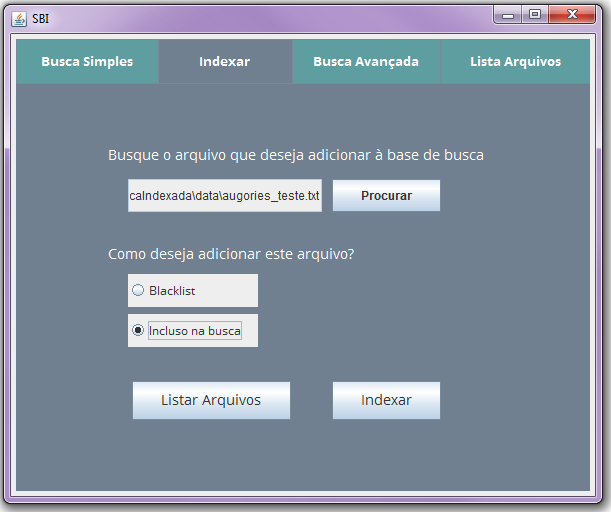
\includegraphics[width=.9\textwidth]{img/tela2-preenchida.png}
\caption{Interface para inserção de arquivos}
\label{fig:insercaoArquivos}
\end{figure}



\subsection{Listagem de Arquivos}
O usuário tem acesso a uma interface que contém uma lista com todos os arquivos adicionados no sistema, nela é possível encontrar o nome deles ordenados em ordem alfabética, bem como a quantidade de palavras que cada arquivo possui, ver Figura~\ref{fig:listagemArquivos}.

\begin{figure}[!htb]
\centering
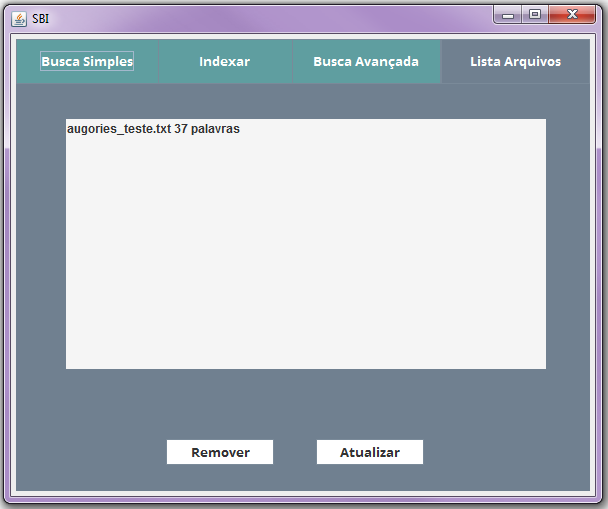
\includegraphics[width=.9\textwidth]{img/tela4-listaArquivos.png}
\caption{Interface para Listagem de arquivos}
\label{fig:listagemArquivos}
\end{figure}

\newpage

\subsection{Remoção de Arquivos}
O sistema permite ao usuário remover arquivos que foram anteriormente adicionados com as palavras que são consideradas pelo mecanismo de busca. Para tanto, por meio da interface gráfica de listagem dos arquivos, o usuário pode selecionar o arquivo que deseja remover e acionar o mecanismo de remoção.

	Quando uma chamada de remoção é feita, o sistema busca todas as palavras associadas ao arquivo selecionado e remove os nós ou índices associados na árvore digital Trie, que armazena das palavras.

\subsection{Atualização de Arquivos}
Quando um arquivo é adicionado uma vez ao sistema, não é permitido que seja adicionado novamente, a menos que tenha sido excluído. Assim, caso o conteúdo do arquivo seja alterado, as novas palavras (se existiram) não serão incluídas na estrutura e, portanto, não serão vistas pelos mecanismos de busca.

	Para isso, na interface de listagem dos arquivos o usuário pode selecionar um arquivo e acionar a atualização. Desta forma, o sistema verifica se há alguma palavra no arquivo que não está adicionada na estrutura de dados e a inclui.

\subsection{Busca de Palavras}
Há três tipos de busca que podem ser realizadas: \\
$\bullet$ Busca Simples\\
$\bullet$ Busca AND\\
$\bullet$ Busca OR

Há duas interfaces gráficas correspondentes à busca. Na inicial, o usuário tem um campo de texto no qual uma palavra pode ser digitada. Ao acionar o mecanismo de busca, a palavra é buscada na árvore digital Trie, levando em consideração o tipo Busca Simples e o resultado é listado logo acima do buscador.

	Há uma interface gráfica de busca avançada, na qual a organização segue a mesma da inicial, contudo é permitido ao usuário a busca por mais de uma palavra, possibilitando acionar o tipo Busca AND ou Busca OR. Na AND, são listados apenas os arquivos que contém todas as palavras solicitadas na busca, enquanto na OR são exibidas todas as ocorrências que contém as palavras, não necessariamente todas que foram solicitadas.

\subsection{Listagem do resultado da(s) palavra(s) buscada(s)}
Na mesma interface que é permitido acionar a busca por palavras, há um campo reservado para a listagem com os resultados. Assim, quando o usuário aciona a funcionalidade de busca, automaticamente é chamada a função de listagem dos resultados, que lista, na interface, o resultado encontrado.

	O formato da listagem dos resultados segue apresentando o título do arquivo está associada, a quantidade de ocorrências identificadas da palavra buscada (na mesma linha) e a linha do arquivo na qual ela se encontra, ver Figura~\ref{fig:formatoListagem}.

\begin{figure}[!htb]
\centering
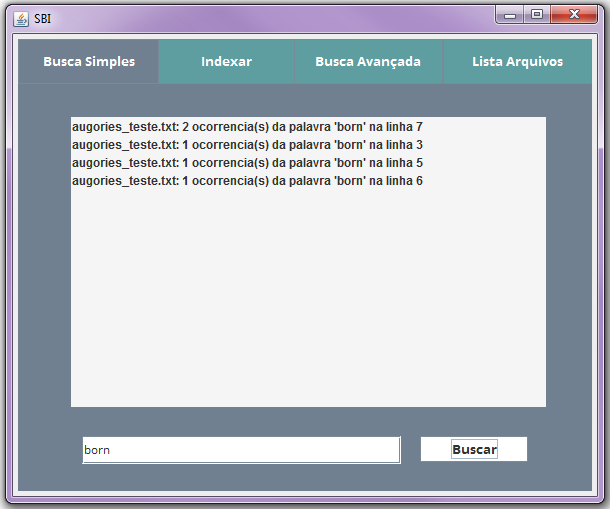
\includegraphics[width=.87\textwidth]{img/tela1-preenchida.png}
\caption{Listagem das palavras encontradas}
\label{fig:formatoListagem}
\end{figure}

\section{Descrição da solução}
 
 Para solucionar os problemas e desafios encontrados para implementar a aplicação descrita, foram tomadas algumas decisões. Quatro opções de menu são exibidas para o usuário: Busca Simples, Indexar, Busca Avançada e Listar Arquivos. Por meio dessas telas é possível utilizar todas as funcionalidades do sistema. 
 
Na aba da busca Simples, é possível pesquisar uma palavra simples na base de texto, os resultados encontrados são exibidos em uma caixa de texto logo acima da caixa de busca, ver Figura~\ref{fig:formatoListagem}.

Para inserir um novo arquivo na base de dados é preciso acessar a aba Indexar. Quando um novo arquivo é inserido, uma classe chamada Engine é responsável por todo o processamento do texto. Primeiramente ele chama a classe Parser, que é responsável por separar cada palavra e informar o arquivo que ela pertence e a linha em que foi encontrada. Feito isso, a engine adiciona essas informações na estrutura de dados escolhida. Caso um arquivo não possa ser lido, uma mensagem informando isto é mostrada, caso contrário, uma mensagem de sucesso é exibida. Para facilitar a escolha de um arquivo, um componente da interface Java mostrando os arquivos e pastas do usuário é exibido, ver Figura~\ref{fig:procurarArquivos}. 

\begin{figure}[!htb]
\centering
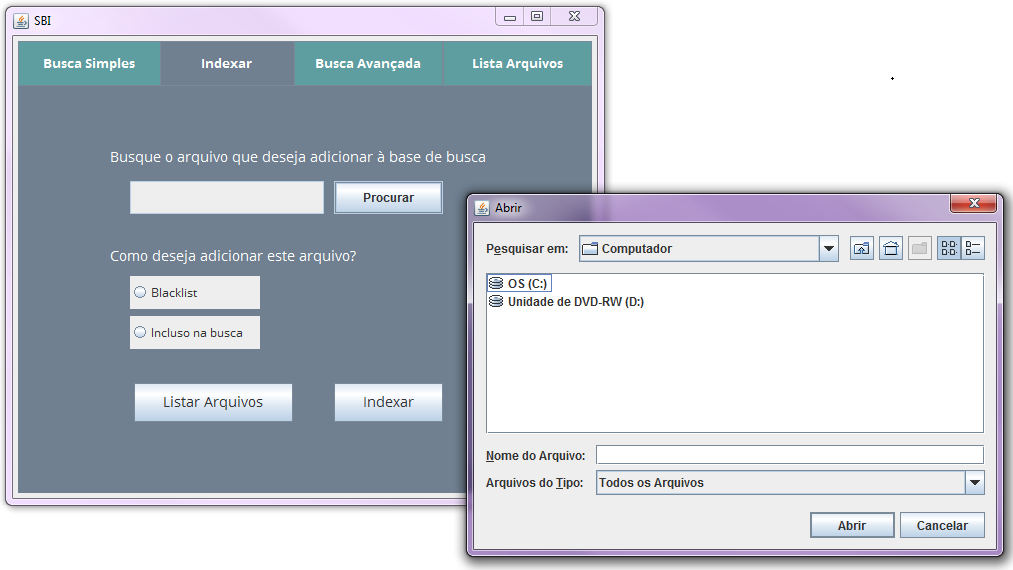
\includegraphics[width=.9\textwidth]{img/telaProcurarArquivo.png}
\caption{Interface para buscar arquivos e adicionar na base de dados}
\label{fig:procurarArquivos}
\end{figure}

	Para o armazenamento das informações que o sistema usa, foi criado uma classe DataBase, ela possui a lista de arquivos que foram inseridos e a árvore Trie que possui  todas as palavras dos respectivos arquivos. Para a implementação da classe Trie, criou-se duas classes auxiliares, Node e Index, que podem lançar exceções representadas pela classe TreeException. A classe Node representa um nó da árvore e a classe Index um índice de palavra, este é constituído por uma linha, um arquivo e quantidade de ocorrências de uma palavra na linha do arquivo. Quando um nó é dito terminal, ele representa o último caracter de uma palavra, esse nó, então, armazena uma lista de índices que contém todas as ocorrências encontradas nos arquivos adicionados.
	
	Para representar as buscas uma classe abstrata Search foi criada, as demais classes (SearchAnd e SearchOr) herdam dessa classe e implementam a busca específica que elas representam. Com relação aos dados coletados pelas buscas, eles são ordenados de acordo com os seguintes critérios: a lista exibe as ocorrências das palavras pesquisadas na ordem em que foram inseridas, por exemplo, quando se busca as palavras “informática” e “empresa”, primeiro são mostradas as ocorrências da palavra “informática” e depois de “empresa”. Sobre a exibição das ocorrências de uma palavra, primeiro é listado os arquivos com mais palavras encontradas, as linhas com mais ocorrências vêm primeiro, ver Figuras ~\ref{fig:buscaOrResultados} e ~\ref{fig:buscaAndResultados}. 

\begin{figure}[!htb]
\centering
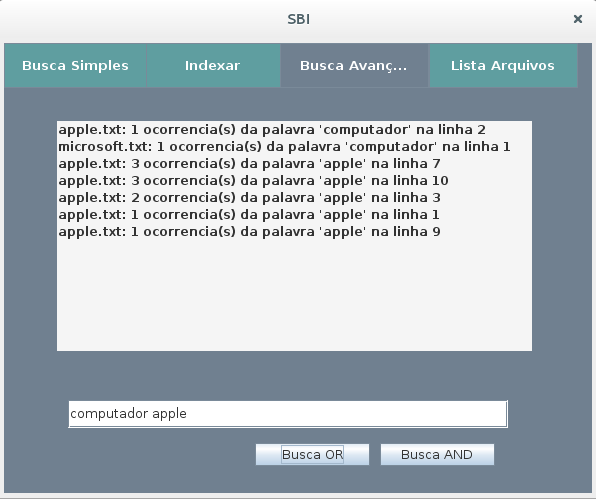
\includegraphics[width=.9\textwidth]{img/buscaOr.png}
\caption{Resultados exibidos de uma busca do tipo OR}
\label{fig:buscaOrResultados}
\end{figure}

\begin{figure}[!htb]
\centering
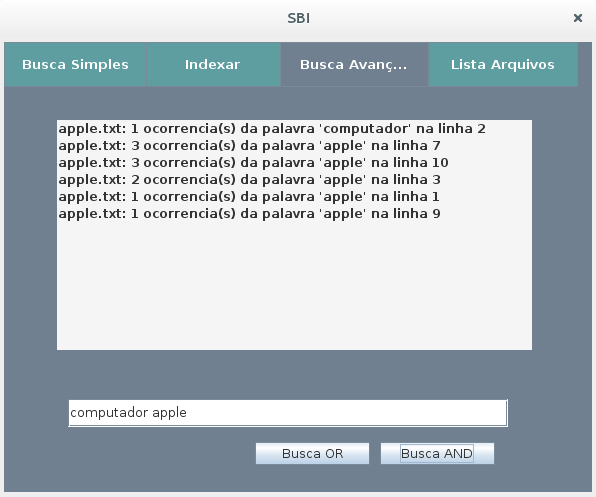
\includegraphics[width=.9\textwidth]{img/buscaAnd.png}
\caption{Resultados exibidos de uma busca do tipo And}
\label{fig:buscaAndResultados}
\end{figure}

\newpage

	Para coordenar todas as opções do sistema, uma classe principal SearchSystem foi criada, que é o intermédio de comunicação entre a aplicação e o usuário. Basicamente sua função é montar a interface do sistema e faz com que as solicitações sejam enviadas para as classes responsáveis por executar tal ação. Para a interface gráfica, cada seção da interface com o usuário herda de uma interface principal ViewSBI, a qual é relacionada com a SearchSystem ver Figura~\ref{fig:diagramaDeClasses}.


\begin{figure}[!htb]
\centering
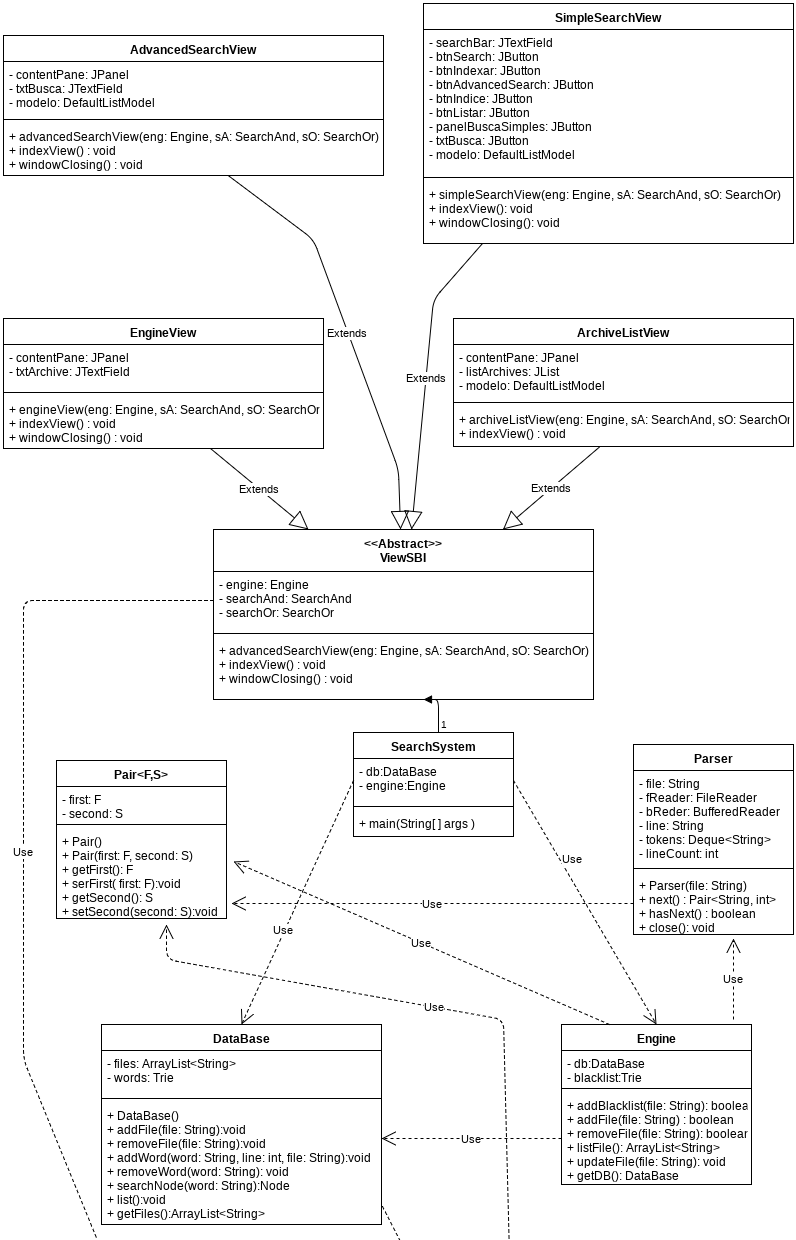
\includegraphics[width=.96\textwidth]{img/sbi_project-part1.png}
\end{figure}
\begin{figure}[!htb]
\centering
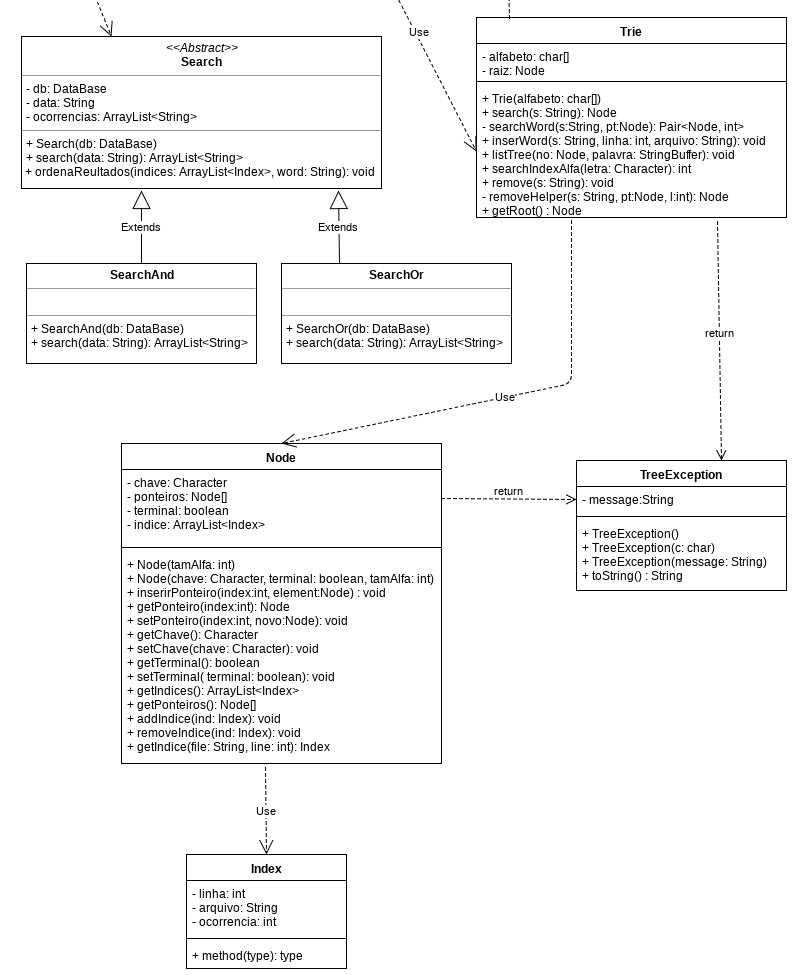
\includegraphics[width=.96\textwidth]{img/sbi_project-part2.png}
\caption{Diagrama de Classes do Sistema}
\label{fig:diagramaDeClasses}
\end{figure}
  
 \newpage
 
\section{Estruturas de Dados}

A estrutura de dados escolhida para a implementação deste tipo de sistema foi a árvore digital Trie. Essa estrutura permite realizar a busca por uma palavra em $O(k\times log(m))$, onde $k$ é o tamanho da chave buscada e $m$ é o número de caracteres no alfabeto.

A principal característica de uma árvore digital é que uma chave não é mantida em um único nó, mas sim obtida através de uma sequência de nós que começa da raiz e vai até um determinado nó v que é denominado terminal. Além disso, o caminho da raiz até um nó qualquer é chamado de prefixo. 

Cada nó corresponde a um único dígito e a aresta entre o próprio nó e seu pai representa o caractere que compõe a chave. Para implementar a estrutura de acordo com esta propriedade, é utilizada uma árvore m-ária e a recuperação/atribuição do caractere é feita uma busca binária para definir cada filho do nó.

Dessa forma, ao buscar uma palavra no sistema, não é feita a comparação de toda a chave em cada nó, o que resultaria em $O(log(n))$ comparações e cada operação geraria um custo proporcional ao comprimento da palavra, mas sim de cada dígito que forma o prefixo da chave na Trie. É essa particularidade que torna a árvore digital mais eficiente para este tipo de aplicação que as demais.

Na implementação da busca para o sistema, primeiramente são realizadas $k$ interações, sendo $k$ o tamanho da chave a ser procurada, para percorrer o caminho formado pelos dígitos da palavra buscada. Em cada passo desse percurso, é realizada a busca do índice do próximo nó a ser visitado e a atualização do ponteiro. Essa busca é feita no próprio alfabeto, que, por ser mantido em um vetor ordenado, possibilita a busca binária do índice. Ao final do laço, é verificado se o último ponteiro é, de fato, terminal. Assim, o algoritmo possui complexidade $O(k\times log(m))$, onde $m$ é o tamanho do alfabeto definido.

Para facilitar o armazenamento das ocorrências de uma certa palavra nos arquivos do sistema, cada nó terminal carrega também a informação de em quais arquivos a contém, bem como as linhas e o número de vezes que o termo se repete.


\section{Reflexão}
Ao longo da disciplina, foi aprendido sobre a importância de efetuar um bom planejamento do projeto, com discussões sobre o que precisa ser desenvolvido, descrição das principais funcionalidades, antes da implementação, e elaboração de um diagrama de classes do sistema.

O projeto foi desenvolvido levando em consideração essas abordagens. Deste modo, antes de iniciarmos a codificação, foi feito um levantamento das funcionalidades que o sistema deveria ter, descrição e investigação sobre a relação entre as classes e funções que poderiam ser utilizadas por mais de uma funcionalidade, bem como o modo como isso seria visualizado (interfaces gráficas). Além disso, foi elaborado um diagrama de classes inicial para o sistema.

Após isso, foi gerado e documentado uma versão inicial (stub) das classes do sistema, com a declaração e descrição da composição (campos e comportamentos) de cada uma das  classes que foram planejadas no diagrama de classes. Essas primeiras etapas do projeto foram realizadas com a equipe reunida e, depois de concluído, houve a divisão de tarefas entre os membros do grupo.

A implementação do sistema foi realizada utilizando como suporte uma ferramenta apresentada em sala: o sistema de controle de versão de arquivos (git) e o sistema de hospedagem de projetos (github), que possui, também, funções extras aplicadas ao git.

Quanto ao desenvolvimento do sistema, um dos problemas que não foi solucionado é o da implementação do autocorrect, isto é, a identificação de palavras semelhantes à que foi digitada na busca, de modo a tratar erros como o de digitação incorreta por parte do usuário.

Outro ponto que poderia ser melhorado é que, pelo fato da árvore Trie possuir ponteiros para vários outros nós, sua utilização implica em um consumo de memória considerável. Um meio de solucionar esse problema é o uso de tabelas hash para armazenar os nós filhos ao invés de simplesmente um vetor, diminui o espaço ocupado por um único nó. Outra alternativa é a implementação da árvore Patrícia, que é uma variação da Trie na qual os nós que possuem apenas um filho são comprimidos de forma a representar uma substring, e não mais apenas um dígito.

Além disso, não foi implementada uma classe de validação dos arquivos, logo, arquivos
que não estão no formato aceito lançam uma exceção, ao invés de serem tratados e impedirem a adição ao repositório. 

\section{Bibliografia}

\setlength{\parindent}{0cm}
BARNES, David J.; KÖLLING, Michael. Programação Orientada a Objetos com Java: Uma introdução prática usando o BlueJ. 4. ed. São Paulo: Pearson, 2009.

CORMEN, Thomas H. et al. Algoritmos: Teoria e Prática. 2. ed. Rio de Janeiro: Elsevier, 2002. (6º Reimpressão).

SZWARCFITER, Jayme Luiz; MARKENZON, Lilian. Estruturas de Dados e seus Algoritmos. 2. ed. Rio de Janeiro: Ltc, 1994.

\end{document}